\documentclass[10pt,a4paper]{article}
\usepackage[margin=0.9in]{geometry}
\usepackage[T1]{fontenc}
\usepackage{lmodern}
\usepackage{booktabs}
\usepackage{graphicx}
\usepackage{url}
\title{NIST P-256 / P-384 Pollard rho on one RTX PRO 6000:\\
       the ECC2K-130 GPU ladder applied to prime fields}
\date{2026-10-13}
\author{}
\begin{document}
\maketitle

\paragraph{What this is.} A copy, for browsing, of the measurements behind
Section~7 of the ECC2K-130 paper (\path{paper/ecc2k130/}). The source of
truth is \path{gpu/nist/RESULTS.md} (round 1 on \texttt{main}) and its
round-2 update in aburan28/crypto pull request 1778 (open at the time of
writing). This report computes nothing new: every value below is copied
from those records, and ratios are quotients of two recorded values.

\paragraph{Setup (as recorded).} One NVIDIA RTX PRO 6000 Blackwell Server
Edition (cc~12.0, 188 SMs), CUDA~13.3, \texttt{-arch=sm\_120}, run on Modal
through \path{gpu/nist/modal_app.py}. Walk: $r$-adding Pollard rho with the
negation-map fold, distinguished points at probability $2^{-24}$, $W$ walks
per thread sharing one Fermat inversion, CIOS Montgomery field with $n'=1$.
Each sweep cell is one run of $8{,}192$ iterations. Modal runs: PTX build
\texttt{ap-39mdjitYFxkMRHk6pFdd2P}, round-1 sweep
\texttt{ap-o766pq9fqlurbzSYcqZoe6}, round-2 sweep
\texttt{ap-0KNqNM8D1J4YQn5z67Ucc0} (timed out at Modal's 4~h limit during the
last \texttt{maxreg=160} cells; every reported cell completed).

\paragraph{Correctness on the device.} Distinguished-point counts matched
$\text{walks}\times\text{iterations}/2^{24}$ in every cell (for example
$11{,}969$ observed against $12{,}085$ expected on the first P-256 run;
$12{,}154$ against $12{,}096$ in the best cell). The CPU suite cross-checks
the compile-time-$W$ stepper bit for bit against the generic stepper.

\begin{figure}[h]
\centering
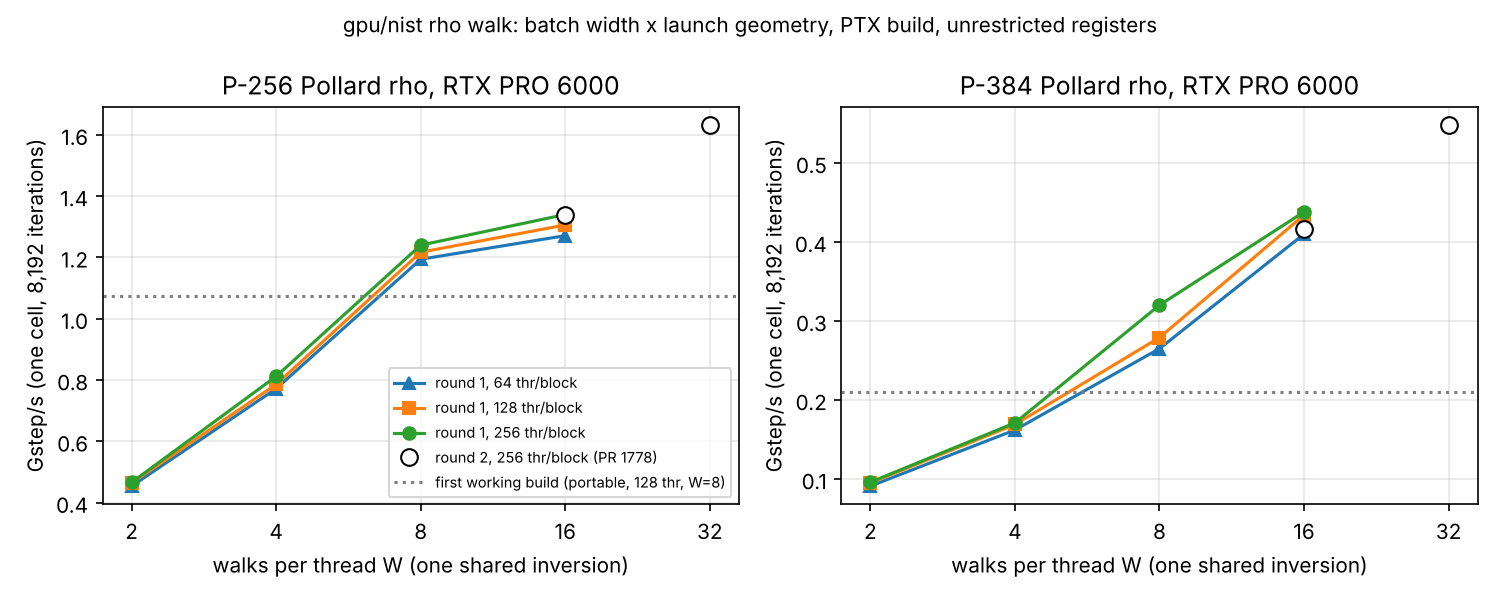
\includegraphics[width=\textwidth]{nist_rho_w_sweep.png}
\caption{Recorded rho rates against the batch width $W$ for three launch
  geometries (round 1) and the round-2 cells at 256 threads per block,
  unrestricted registers. Dotted line: first working build (portable, 128
  threads, $W=8$). Data: \path{data.csv}; plot: \path{plot.py}.}
\end{figure}

\begin{table}[h]
\centering
\small
\begin{tabular}{@{}llrr@{}}
\toprule
step & cells compared & P-256 & P-384 \\
\midrule
first working build & portable, 128 thr., $W=8$ & 1.075 & 0.210 \\
explicit PTX carry chains & same cell, PTX & 1.282 ($1.19\times$) & 0.289 ($1.38\times$) \\
$W=8\to16$ & 256 thr., PTX & 1.24 $\to$ 1.340 & 0.32 $\to$ 0.438 \\
$W=16\to32$, by-ref.\ inversion (PR 1778) & 256 thr., PTX & 1.339 $\to$ 1.632 & 0.417 $\to$ 0.548 \\
register caps 96/128/160 (PR 1778) & 256 thr., $W=32$ & 1.589--1.595 & 0.447--0.455 \\
\midrule
best cell, cumulative & PTX, 256 thr., $W=32$ & \textbf{1.632 (1.52$\times$)} & \textbf{0.548 (2.61$\times$)} \\
\bottomrule
\end{tabular}
\caption{Rates in Gstep/s. Class: engineering; the step count is unchanged
  and $S=\text{steps}/\sqrt n$ is flat.}
\end{table}

\paragraph{Limits.} The cells are single runs, not interleaved repeated
pairs, so no interval is available for any ratio. The round-2 gain cannot
be split between the larger batch and the by-reference inversion because
round 1 never compiled $W=32$; at $W\le16$ the two rounds agree within
noise. A Solinas-field walk was not built. At $1.63$~Gstep/s a P-256
collision needs about $1.9\cdot10^{30}$~s: these are throughput
measurements, not a statement about the security of the NIST curves.

\end{document}
